\subsection{FGR Background}
%%%%%%%%%%%%%%%%%%%%%%%%%%%%%%%%%%%%%%%%%%%%%%%%%%%%%%%%%%%%%%%%%%%%%%%%%%%%%%%%%%%%%%%%
\begin{frame}
\frametitle{High Level Overview}

\begin{itemize}
  \item Fission reactions in $UO_2$ fuel generate the gases Xe and Kr in the fuel grains.
  \item Through a diffusive process these fission gases reach the grain face and begin to form bubbles.
  \item The bubbles increase in size as fission gases accumulate. Eventually, the bubbles coalesce and form multilobed pores.
  \item When bubbles come into contact with the grain edges gas is released from the grain faces.
\end{itemize}

\end{frame}
%%%%%%%%%%%%%%%%%%%%%%%%%%%%%%%%%%%%%%%%%%%%%%%%%%%%%%%%%%%%%%%%%%%%%%%%%%%%%%%%%%%%%%%%
\begin{frame}
\frametitle{Understanding Thermal FGR is Critical for Reactor Safety}

\begin{itemize}
  \item On one hand, if the Xe and Kr gases remain in the fuel matrix the fuel will swell.
  \item Potential result is clad damage or failure as contact pressure between fuel and clad increases.
  \item On the other hand, release of fission gases into rod free volume reduces the thermal conductivity of the fuel-clad gap and contributes to high operating pressures.
  \item Can result in clad lift-off and dangerous fuel temperature swings. 
\end{itemize}

\end{frame}
%%%%%%%%%%%%%%%%%%%%%%%%%%%%%%%%%%%%%%%%%%%%%%%%%%%%%%%%%%%%%%%%%%%%%%%%%%%%%%%%%%%%%%%%
\begin{frame}
\frametitle{FGR in Pictures}

\begin{columns}
 \begin{column}{0.5\textwidth}
  \centering
  Early Bubble Formations 
  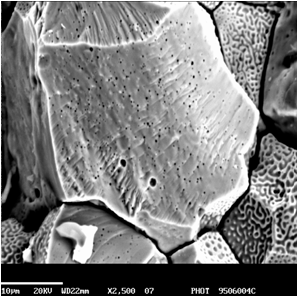
\includegraphics[width=1.\textwidth]{./fgr_3.png}
 \end{column}
 \begin{column}{0.5\textwidth}
  \centering
  Bubble Coalescence
  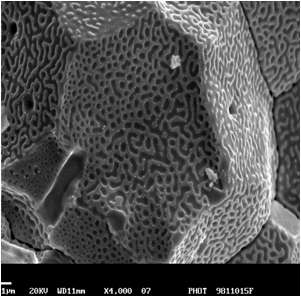
\includegraphics[width=1.\textwidth]{./fgr_2.png}
 \end{column}
\end{columns}

\footnotetext[1]{\tiny G. Pastore, D. Pizzocri, J.D. Hales, S.R. Novascone, D.M. Perez, B.W. Spencer, R.L. Williamson, P. Van Uffelen, L. Luzzi, Modelling of Transient Fission Gas Behaviour in Oxide Fuel and Application to the BISON Code, Enlarged Halden Programme Group Meeting, Røros, Norway, September 7-12, 2014.}

\end{frame}
%%%%%%%%%%%%%%%%%%%%%%%%%%%%%%%%%%%%%%%%%%%%%%%%%%%%%%%%%%%%%%%%%%%%%%%%%%%%%%%%%%%%%%%%
\begin{frame}
\frametitle{FGR in Pictures}

\begin{columns}
 \begin{column}{0.5\textwidth}
  \centering
  Multi-lobed Pores 
  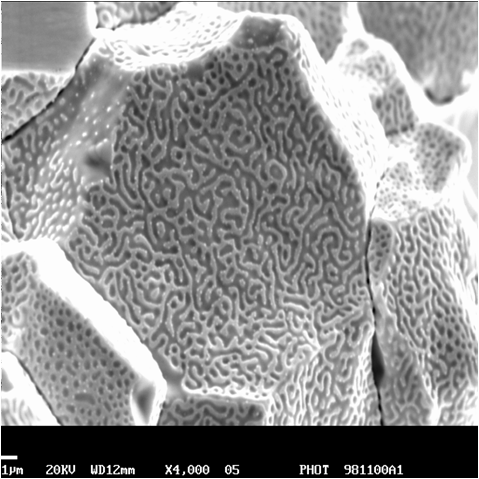
\includegraphics[width=1.\textwidth]{./fgr_1.png}
 \end{column}
 \begin{column}{0.5\textwidth}
  \centering
  Gas Release
  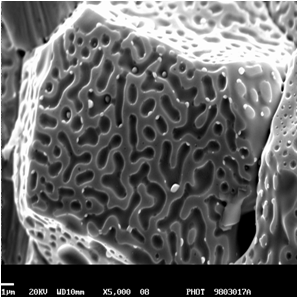
\includegraphics[width=1.\textwidth]{./fgr_4.png}
 \end{column}
\end{columns}

\footnotetext[1]{\tiny G. Pastore, D. Pizzocri, J.D. Hales, S.R. Novascone, D.M. Perez, B.W. Spencer, R.L. Williamson, P. Van Uffelen, L. Luzzi, Modelling of Transient Fission Gas Behaviour in Oxide Fuel and Application to the BISON Code, Enlarged Halden Programme Group Meeting, Røros, Norway, September 7-12, 2014.}

\end{frame}
%%%%%%%%%%%%%%%%%%%%%%%%%%%%%%%%%%%%%%%%%%%%%%%%%%%%%%%%%%%%%%%%%%%%%%%%%%%%%%%%%%%%%%%%
\begin{frame}
\frametitle{Modeling FGR: Intra-granular Gas Diffusion}

\begin{itemize}
  \item Describes how fission gases are transported from fuel grain to fuel face. 
  \item The resolution parameter $b$ describes the rate at which gas bubbles are destroyed due to irradiation and sent back into the fuel lattice.
  \item $D_s$ is the single gas atom diffusion coefficient in a $UO_2$ lattice.
\end{itemize}

\begin{equation}
 \frac{dC_{ig}}{dt} = \frac{b}{b+g}D_s \frac{1}{r^2} \frac{\partial}{\partial r} \left(r^2 \frac{\partial C_{ig}}{\partial r} \right) +\beta \nonumber
\end{equation}

\end{frame}
%%%%%%%%%%%%%%%%%%%%%%%%%%%%%%%%%%%%%%%%%%%%%%%%%%%%%%%%%%%%%%%%%%%%%%%%%%%%%%%%%%%%%%%%
\begin{frame}
\frametitle{Modeling FGR: Bubble Growth}

\begin{itemize}
  \item As gas atoms diffuse to the fuel grain boundary they get absorbed into bubble nuclei. 
  \item The bubbles grow/shrink due to the absorption/emission of vacancies. Fission gas is mainly retained in the bubbles.   
\end{itemize}

\begin{equation}
 \frac{dV_{gf}}{dt} = \omega\frac{dn_g}{dt} + \Omega_{gf}\frac{dn_v}{dt}  \nonumber
\end{equation}  

\end{frame}
%%%%%%%%%%%%%%%%%%%%%%%%%%%%%%%%%%%%%%%%%%%%%%%%%%%%%%%%%%%%%%%%%%%%%%%%%%%%%%%%%%%%%%%%
\begin{frame}
\frametitle{Modeling FGR: Bubble Growth}

\begin{equation}
 \frac{dn_v}{dt} = \frac{2\pi D_v \delta_g}{kTs}\left(p - p_{eq}\right) \nonumber
\end{equation}   

\begin{itemize}  
  \item $D_v$ is the vacancy diffusion coefficient, $T$ is the fuel temperature.
  \item The pressure $p_{eq}$ acting on the bubble is given as the difference between the bubble surface tension $\gamma$ and the hydrostatic stress $\sigma_h$ of the surrounding medium.
  \item Mechanical equilibrium requires that the pressure of the gas in the cavity be balanced by the bubble capillarity.
\end{itemize}

\begin{equation}
 p_{eq} = \frac{2\gamma}{R_{gf}} - \sigma_h \nonumber
\end{equation} 

\end{frame}
%%%%%%%%%%%%%%%%%%%%%%%%%%%%%%%%%%%%%%%%%%%%%%%%%%%%%%%%%%%%%%%%%%%%%%%%%%%%%%%%%%%%%%%%
\begin{frame}
\frametitle{Modeling FGR: Bubble Coalescence}

\begin{itemize}  
  \item As the grain face bubbles begin to grow, they'll coalesce. 
  \item Under the assumption of uniform bubble size and the conservation of total bubble volume, the relationship between the bubble number density $N_{gf}$ and projected area on the grain face $A_{gf}$ is:

\begin{equation}
 \frac{dN_{gf}}{dt} = -\frac{6N_{gf}^2}{3+4n_{gf}A_{gf}} \frac{dA_{gf}}{dt} \nonumber
\end{equation}

\end{itemize}

\end{frame}
%%%%%%%%%%%%%%%%%%%%%%%%%%%%%%%%%%%%%%%%%%%%%%%%%%%%%%%%%%%%%%%%%%%%%%%%%%%%%%%%%%%%%%%%
\begin{frame}
\frametitle{Modeling FGR: Grain Face Saturation}

\begin{itemize}  
  \item Thermal FGR occurs when the grain face saturation condition holds.

\begin{equation}
 \frac{d\left(N_{gf} A_{gf}\right)}{dt} = 0 \nonumber 
\end{equation}
  
  \item The rate of thermal release is:

\begin{equation}
 \frac{dC_{thr}}{dt} = \frac{3}{r_{gr}}\left(1 - P_f\right) \frac{d\psi_{thr}}{dt}  \nonumber
\end{equation} 

  \item The factors $r_{gr}$ and $P_f$ represent the fuel grain radius and fuel porosity, respectively. 

\end{itemize}

\end{frame}
%%%%%%%%%%%%%%%%%%%%%%%%%%%%%%%%%%%%%%%%%%%%%%%%%%%%%%%%%%%%%%%%%%%%%%%%%%%%%%%%%%%%%%%%
\begin{frame}
\frametitle{Modeling FGR: Implementation}

\begin{itemize}  
  \item The FGR model described here has been implemented and validated in the finite element-based fuel performance modeling code Bison by Pastore et. al.
  \item Bison is used to model the Ris\o~AN3 FGR kinetics.
  \item Due to the relatively high temperatures involved in the Ris\o~AN3 power ramp experiment athermal FGR is trumped by its thermal counterpart. 
  \item Bison reports integral fission gas release values. Being a finite element code, Bison computes the gas release at each integration point. 
  \item The ratio of total fission gas released into the rod free volume to the total fission gas generated at each integration point is the quantity of interest in this work.
\end{itemize}

\end{frame}
%%%%%%%%%%%%%%%%%%%%%%%%%%%%%%%%%%%%%%%%%%%%%%%%%%%%%%%%%%%%%%%%%%%%%%%%%%%%%%%%%%%%%%%%




